\documentclass[10pt]{article}
\usepackage[T1]{fontenc}
\usepackage{lmodern,amsmath,amssymb,graphicx,hyperref}
\usepackage[margin=.74in]{geometry}
\setlength{\parindent}{0pt}\setlength{\parskip}{7pt}
\begin{document}
\begin{center}{\Large Actual right-entry quotient and creation coordinates}\\[4pt]
Local continuation --- 15 November 2026\end{center}
\textbf{Result.} The actual scalar word entry is now bound to a concrete
retained-polynomial quotient and nilpotent-variable quotient. Its value equals
evaluation of the canonical reduced actual absoluteRight polynomial. Explicit
normal-coordinate identities then show that padding the creation words at a
later precision reuses the same coordinate integers [pcc:unverified].

\textbf{Local evidence.} Accepted072 has360 theorem statements including
parent344, hence16 new component statements. It exits0 without warnings or
sorryAx. Receipt037 binds exact source, raw compiler output and exit. Data
PCC-20261115-f8ad53 records that local observation. Central printed
dependencies are standard. This is outside shared Transport53/57/fresh
coverage; the records are unsigned and defaultnot\_covered [pcc:unverified].

\textbf{Constructed rings.} For a retained integer polynomial $f$, define
\[
 R_{p_c}=\mathbb Z/2^{p_c}\mathbb Z,\qquad
 B_{p_c}=R_{p_c}[U]/(\bar f),\qquad
 A_{p_c}=B_{p_c}[V]/(V^\ell).
\]
Here $\bar f$ is obtained by mapping the same integer coefficients modulo
$2^{p_c}$. Both quotients use pinned Mathlib AdjoinRoot, with explicit scalar
maps and the actual adjoined nilpotent $v$. The proof derives $v^\ell=0$;
there is no supplied favorable root. If $p_c>0$ and $f$ is monic of positive
degree, the coefficient quotient is proved nontrivial. This does not prove
irreducibility or construct the original binary irreducible-polynomial search
[pcc:unverified].

\textbf{Finite evaluation.} For any polynomial $Q$, ring map $g$ and
$z^\ell=0$, the proof establishes
\[
 Q.\operatorname{eval}_2(g,z)=
 \sum_{n<\ell}g(Q_n)z^n.
\]
It uses the actual finite polynomial expansion and nilpotence; coefficients
above the cutoff vanish after evaluation. Empty cutoffs are retained
algebraically, although the nontrivial original representation requires its
own positive dimension premises [pcc:unverified].

\textbf{Actual coefficient driver.} Let $w_n$ be the output word of the
previous completeEntry routine at $p_c$ and coefficient index $n$. Define
\[
 E=\sum_{n<\ell}\iota(V_{p_c}(w_n))v^n,
\]
where $V_{p_c}$ is canonical word value and $\iota$ the explicit scalar map
into $A_{p_c}$. The source proves that $E$ equals evaluation of the actual
reduced absoluteRight polynomial, under exactly the previous node, valuation,
label and port hypotheses. No full polynomial is supplied as a runtime input
to the word coefficient routine; the polynomial occurs in the correctness
statement. This result does not yet price coefficient preparation, quotient
arithmetic or the finite evaluation loop [pcc:unverified].

\textbf{Sources.} quotient-source-review-001.json pins Mathlib AdjoinRoot,
monic remainder, finite evaluation and degree facts at revision cfc55fc58714.
The earlier primary creation-contract receipt pins the original text and
native source. KB tools were unavailable and the repository wrapper reported
no executable, so the review used exact primary/repository sources. Standard
algebra is reused; no novelty or external theorem certification is claimed
[pcc:unverified].
\newpage
\begin{center}{\Large Normal coordinates and immutable reuse}\end{center}
\textbf{Explicit normal polynomial.} For actual word coefficients, construct
\[
 N(V)=\sum_{n<\ell}C\bigl(\operatorname{of}_{\bar f}(V_{p_c}(w_n))\bigr)V^n.
\]
Its degree is below $\ell$. The actual entry equals the quotient class of
$N$, and the monic-remainder map returns $N$ itself. At each $n<\ell$, the
coefficient in $B_{p_c}$ is exactly the scalar image of $V_{p_c}(w_n)$.
For positive $p_c$ and positive-degree monic $f$, the inner monic remainder
of that coefficient is its constant polynomial. Thus its normal coordinates
are exactly
\[
 \operatorname{coord}_{n,j}(E)=
 \begin{cases}V_{p_c}(w_n),&j=0,\\0,&j\ne0.\end{cases}
\]
These are derived coordinates of this actual right factor, not a favorable
coordinate oracle [pcc:unverified].

\textbf{Later precision.} For $P\ge p_c$, append $P-p_c$ high zero bits to
each creation word. Keep the same integer $f$ and nilpotent cutoff $\ell$.
The resulting entry in $A_P$ has exactly the same integer representative in
every normal coordinate as the creation entry in $A_{p_c}$. The final theorem
instantiates this construction with actual completeEntry words evaluated at
$p_c$. It never calls completeEntry at $P$ and does not assume the lift is a
ring homomorphism [pcc:unverified].

\begin{center}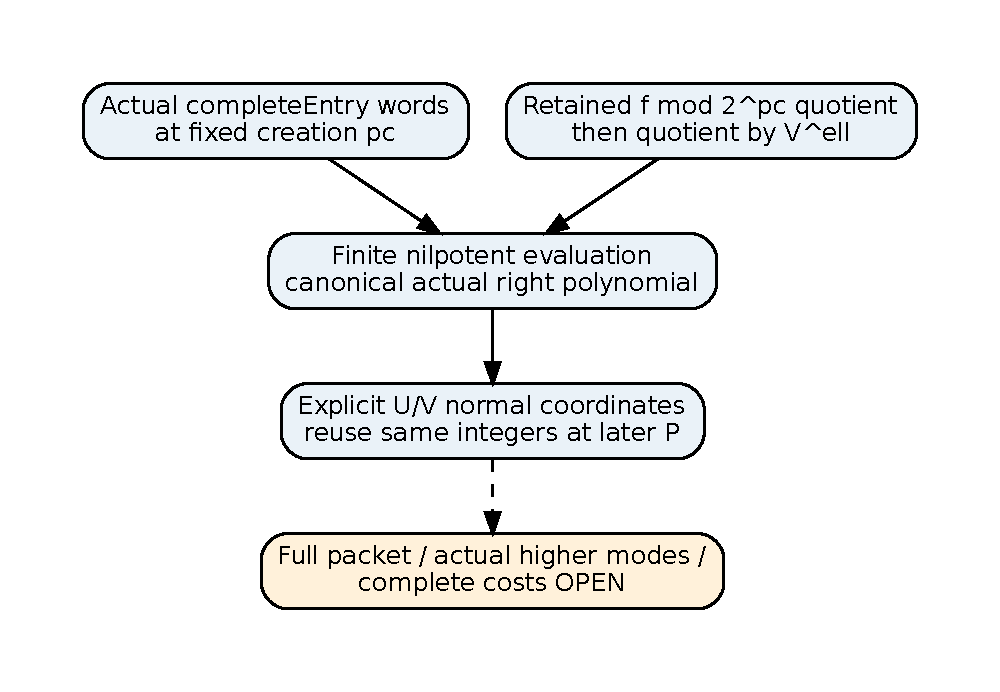
\includegraphics[height=2.8in]{quotient-entry-dependencies-001.pdf}\end{center}

\textbf{Exact scope.} This proves the creation-coordinate contract for the
specific scalar-coefficient right-factor subspace. It does not construct all
extension-valued packet operations, the binary polynomial selector, original
immutable packet metadata or child-entry cost bounds. Scalar preparation,
AST and denominator construction, encoding, control, indices, arrays, trace
concatenation, allocation and memory remain unpriced. Earlier emitted Boolean
arithmetic-event bounds are not total bit runtime [pcc:unverified].

\textbf{Next discriminating obligation.} Count actual nonzero weighted modes,
using coefficient witnesses and support rather than declared capacity. Every
$2^u k$ label remains charged until actual formulas justify pruning. The
separately accepted actual $k=1$ test on the next page proves all $b=0$ labels
have both nonzero factors at a negative pole. Higher degree inventory,
child budgets, the actual elliptic relation, public finder, scalar extraction,
retries and complete expected cost remain separate [pcc:unverified].
\newpage
\begin{center}{\Large Actual zeroth-layer support: no zero pruning}\end{center}
\textbf{Observed proof result.} Accepted074 has367 local statements including
parent360, seven new statements, exit0 and no warnings. Receipt038 pins exact
source, raw output and exit. Central printed dependencies are standard;
shared Transport audit/fresh coverage is not inferred [pcc:unverified].

\textbf{Tested family and hypotheses.} Use the actual compact polynomial
factors polyLeft and polyRight, with $k=1$, retained negative pole
$t=-2^i$, $u\le a$ and $i\le a$. Multiplicities $m_j$ are arbitrary natural
numbers; no positive-anchor hypothesis is added. For each residue label
$r\in\{0,\ldots,2^u-1\}$, set its moment index to $b=0$ and choose the actual
class port with index $r$ on both sides [pcc:unverified].

\textbf{Explicit witnesses.} The completed diagonal polynomial is independent
of the diagonal index. Its actual first chart coefficient, divided by the
nonzero diagonal normalizer, is exactly one. The row numerator preserves this
coefficient because the normalized node constant is zero. At $k=1$ the actual
geometric sum is one. Consequently the constructed factors satisfy
\[
 L_{r,(r,0)}(Z)=1,\qquad [Z^1]R_{(r,0),r}(Z)=1.
\]
Both actual factors therefore have nonzero support. This uses their formulas,
not the declared number of labels or an assumed matrix-rank witness
[pcc:unverified].

\textbf{Exact active set.} Define the finite set by the actual support test
\[
 \mathcal A_0=\{r:\ (\exists x,\ L_{x,(r,0)}\ne0)
                  \land(\exists y,\ R_{(r,0),y}\ne0)\}.
\]
The matching-port witnesses prove
\[
 \mathcal A_0=\{0,\ldots,2^u-1\},\qquad |\mathcal A_0|=2^u.
\]
Thus zero-detection pruning cannot reduce this particular actual zeroth layer.
It is not merely a cardinality bound for a declared label type
[pcc:unverified].

\textbf{Limits and next falsification target.} Nonzero factors need not be
independent. This is not an arbitrary-factor width lower bound, higher-degree
inventory result, full-matrix statement or runtime lower bound. The next
proof obligation is whether the same witness persists for every $k>0$;
then analyze actual $b>0$ coefficient support and valuations. Symmetry and
cancellation may matter, so do not extrapolate all-active support from the
zeroth layer. PROTOCOL-010.md records this continuation [pcc:unverified].

\textbf{Evidence retained.} Failed068--071 and073 sources, raw logs and exits
are preserved alongside accepted072 and074. Compiler elaboration failures
are distinguished from mathematical counterexamples. No native timing,
scaling, paid/cloud or attack campaign was launched. All parent immutable
source, evidence, claim and ledger bytes remain preserved [pcc:unverified].
\end{document}
